%章节
%\section{}, \subsection{}, \subsubsection{}, \paragraph{}, \subparagraph{}

%插入图片
%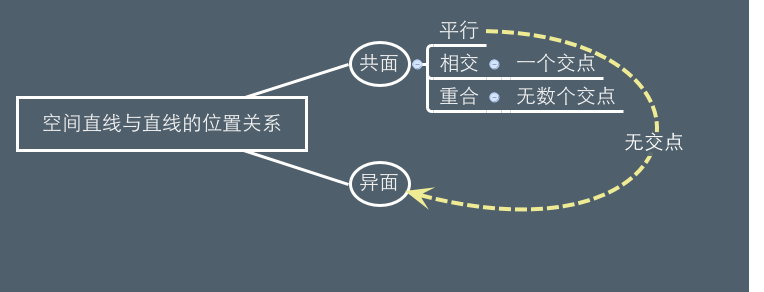
\includegraphics[height=100px]{/Users/shuyue/Desktop/1.png}

%无序列表
%\begin{itemize}
%\item
%\item
%\item
%\item 
%\end{itemize}

%有序列表
%\begin{enumerate}
%\item 
%\item
%\item
%\item
%\end{enumerate}

%嵌套列表
%\begin{itemize}
%\item
%\begin{enumerate}
%\item 
%\item 
%\item 
%\end{enumerate}
%\item
%\begin{enumerate}
%\item 
%\item 
%\item 
%\end{enumerate}
%\end{itemize}

%分栏
%\begin{multicols}{2}
%1\columnbreak \\ 2
%\end{multicols}

%标号
%\textcircled{1}

\documentclass[a4,12pt]{article}
\RequirePackage{CJKutf8,hyperref,mathtools,amssymb,geometry,enumerate,multicol,graphicx}

\begin{document}
\begin{CJK}{UTF8}{gkai}

\title{}
\date{}
\author{张舒悦}
\maketitle

\section{教学目标}
\begin{enumerate}
\item 
\item 
\item 
\end{enumerate}

\section{教学重点}
\begin{enumerate}
\item 
\item 
\item 
\end{enumerate}

\section{教学难点}
\begin{enumerate}
\item 
\item 
\item 
\end{enumerate}

\section{教学过程}

\subsection{引入}

\subsection{例题1}

\subsection{练习1}

\subsection{例题2}

\subsection{练习2}

\section{小结}
\begin{enumerate}
\item
\item
\item
\item 
\end{enumerate}

\section{思考题}
\begin{enumerate}
\item
\item
\item
\item 
\end{enumerate}

\section{作业}
\begin{enumerate}
\item
\item
\item
\item 
\end{enumerate}

\section{板书设计}
\begin{itemize}
\item 
\item
\item
\item
\end{itemize}

\end{CJK}
\end{document}